\section{Building our own tracking system using routers and hotspots}
This section will cover the progress made in building and researching routers and hotspots to make our own Indoor Positioning System (IPS)\sfx{ILBS? IPS? tracking?}. A list of objectives can be seen below. The primary goal is enabling us to calculate our position in geo-coordinates, in order to compare it with the coordinates provided by Cisco MSE.

\begin{itemize}
	\item Equipment Requirements
	\item Test Capabilities of the Router
	\item Test Capabilities of the Access Points
\end{itemize}

\subsection*{Equipment Requirements}
The initial requirement for all equipment is that it supports wireless communication on the 2.4 GHz frequency. It would be advantageous if we set up two different ILBS for the sake of comparison. We decided to buy two brands, allowing us to analyse two ILBS and thus conclude which of the systems performed best, based on the criteria described in section \ref{sec:monitoring}.

Based on the above requirement we found two brands, Ubiquiti and D-link, the latter of which is considered the cheaper brand. We ordered one router, two expensive access points and five cheap access points from each brand.

\subsection*{The physical setup}\ofx{we may want to move this?}
Cisco\cite{access_point_placement} have guidelines for how to place the access points in order to get the best coverage for a system. They recommend that there is an access point in each corner of the building and some along the perimeters. In addition, if the building is large enough, access points should be placed within the perimeter to form a sub-perimeter, which itself may contain a sub-perimeter and so on. This is illustrated on figure \cref{fig:access_placement}, in which the red circles are access points. The perimeter established by the outer-most access points should encapsulate the entire floor, as illustrated by the blue line and the sub-perimeter by the red line. The outer-most perimeter is also known as the \textit{hull}\cite{access_point_placement}.

The access points should be placed at an interval of 50-70 feet to get a high precision without interference and unnecessary overlap\cite{access_point_range}. This radius depends on the reach of the access points and the topology of the building.

\begin{figure}[H]
	\centering
	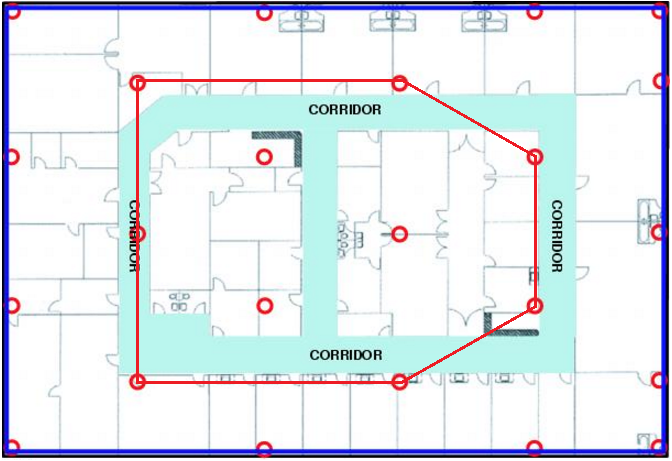
\includegraphics[scale=0.5]{graphics/access_placement.png}
	\label{fig:access_placement}
	\caption{Illustration of how access points should be placed\cite{access_point_placement}.}
\end{figure}

An overview of our system setup can be seen in \cref{fig:OwnSetup}. This setup follows the previous design guidelines. One router is set up in the middle and four access points are set up in our group rooms, such that the system covers three group rooms.

\begin{figure}[H]
	\centering
	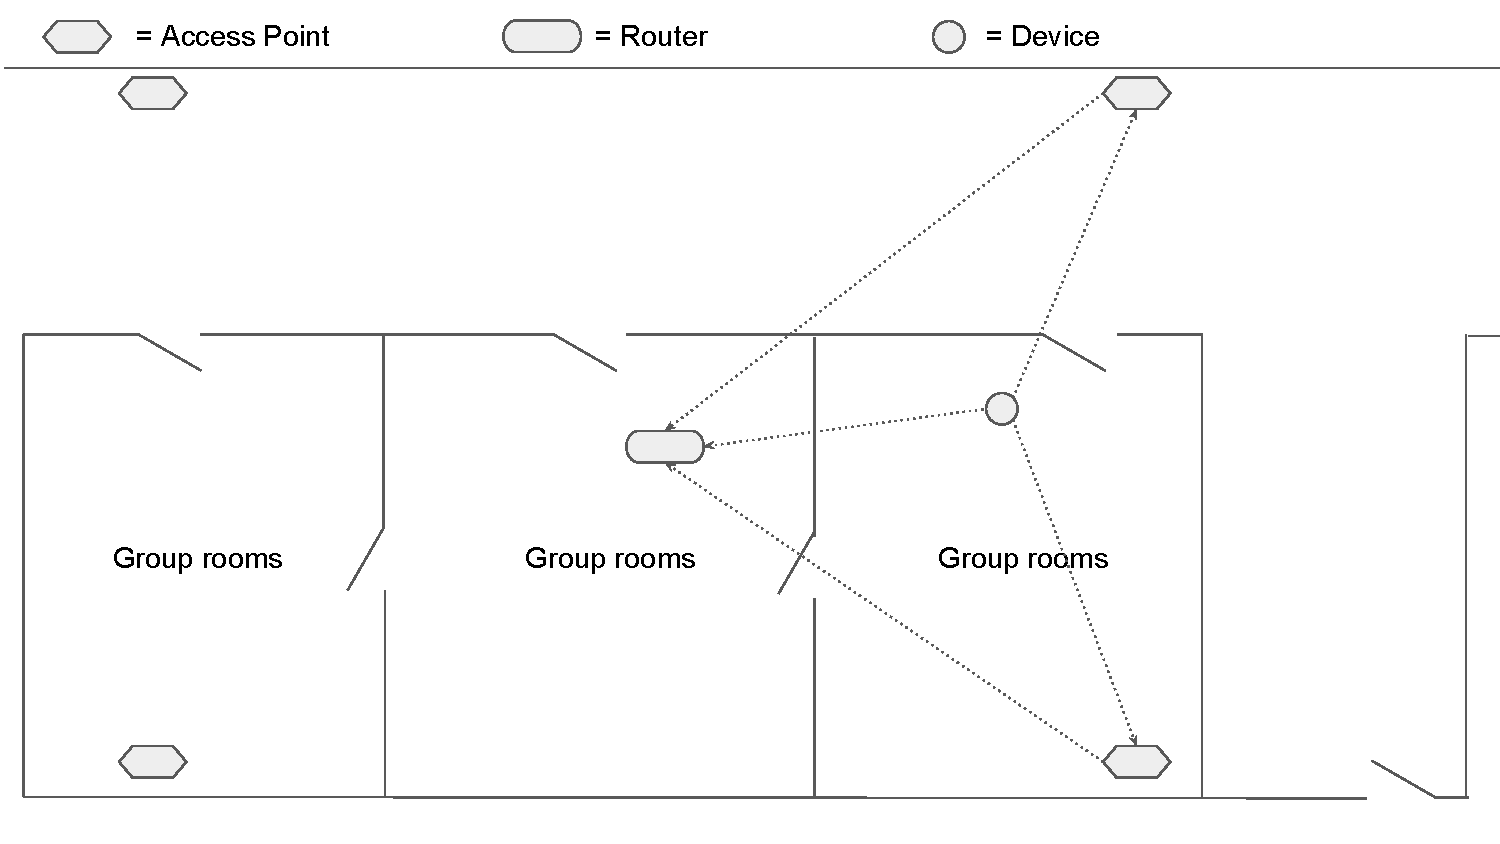
\includegraphics[scale=0.5]{graphics/Router-AccessPoint_Setup.pdf}
	\label{fig:OwnSetup}
	\caption{Illustration of how a positioning system can be set up, using routers and access point that can track devices.}
\end{figure}

\subsection*{Test Capabilities of the Equipment}
We tested the Ubiquiti equipment, with the original firmware. At first glance we are able to get transmission(TX) and receive(RX) signals of connected devices. Unfortunately we do not receive the signals from devices not connected to the network. It was attempted to use the routers terminal which did not yield any results due to restricted access.

This caused us to research custom firmware for the router. By installing new firmware on the router we will be able to get root access to the router, and thereby manipulate it at a lower level than the routers original firmware allows. This is necessary if we are to capture every RX signal the router gets.

We did find custom firmware for Ubiquiti, however not for D-link. These sites we used cover thousands of routers and the fact that we were not able to find a custom firmware for D-link might be because of that particular model, because other routers from the same brand is supported. No conclusion was found as to why it is not covered on any of the websites\cite{firmware_1}\cite{firmware_2}\cite{firmware_3}\cite{firmware_4}\cite{firmware_5}\cite{firmware_6}.

We ended up utilizing the openwrt because it supports our Ubiquiti router and allows us to gain root access and execute programs. With the new custom firmware installed there is roughly 8Mb of free memory left on the router. This put some limitations on which language we can use. Our first attempt is to use a version of python called Mini-Python that does not exceed the memory limit.

A program is constructed allowing us to listen on different types of networks such as LAN and WAN. This is done using the socket library which is a standard library in Python. However, it is not part of the minimalistic version, meaning we had to import it ourselves. We were not able to do this.

\section*{Conclusion}
The progress we have made in building our own tracking system is as following: We were able to update the firmware on the Ubiquiti router, this was required to run programs with root access to use the network interface. With a program running we could get the package information, but it dose not contain the RSSI (Received signal strength indication), this may be because of the network drivers installed on the router, but not confirmation was done. 